\documentclass[]{article}
\usepackage[T1]{fontenc}
\usepackage{lmodern}
\usepackage{amssymb,amsmath}
\usepackage{ifxetex,ifluatex}
\usepackage{fixltx2e} % provides \textsubscript
% use microtype if available
\IfFileExists{microtype.sty}{\usepackage{microtype}}{}
\ifnum 0\ifxetex 1\fi\ifluatex 1\fi=0 % if pdftex
  \usepackage[utf8]{inputenc}
\else % if luatex or xelatex
  \usepackage{fontspec}
  \ifxetex
    \usepackage{xltxtra,xunicode}
  \fi
  \defaultfontfeatures{Mapping=tex-text,Scale=MatchLowercase}
  \newcommand{\euro}{€}
\fi
\usepackage{color}
\usepackage{fancyvrb}
\DefineShortVerb[commandchars=\\\{\}]{\|}
\DefineVerbatimEnvironment{Highlighting}{Verbatim}{commandchars=\\\{\}}
% Add ',fontsize=\small' for more characters per line
\usepackage{framed}
\definecolor{shadecolor}{RGB}{248,248,248}
\newenvironment{Shaded}{\begin{snugshade}}{\end{snugshade}}
\newcommand{\KeywordTok}[1]{\textcolor[rgb]{0.13,0.29,0.53}{\textbf{{#1}}}}
\newcommand{\DataTypeTok}[1]{\textcolor[rgb]{0.13,0.29,0.53}{{#1}}}
\newcommand{\DecValTok}[1]{\textcolor[rgb]{0.00,0.00,0.81}{{#1}}}
\newcommand{\BaseNTok}[1]{\textcolor[rgb]{0.00,0.00,0.81}{{#1}}}
\newcommand{\FloatTok}[1]{\textcolor[rgb]{0.00,0.00,0.81}{{#1}}}
\newcommand{\CharTok}[1]{\textcolor[rgb]{0.31,0.60,0.02}{{#1}}}
\newcommand{\StringTok}[1]{\textcolor[rgb]{0.31,0.60,0.02}{{#1}}}
\newcommand{\CommentTok}[1]{\textcolor[rgb]{0.56,0.35,0.01}{\textit{{#1}}}}
\newcommand{\OtherTok}[1]{\textcolor[rgb]{0.56,0.35,0.01}{{#1}}}
\newcommand{\AlertTok}[1]{\textcolor[rgb]{0.94,0.16,0.16}{{#1}}}
\newcommand{\FunctionTok}[1]{\textcolor[rgb]{0.00,0.00,0.00}{{#1}}}
\newcommand{\RegionMarkerTok}[1]{{#1}}
\newcommand{\ErrorTok}[1]{\textbf{{#1}}}
\newcommand{\NormalTok}[1]{{#1}}
% Redefine labelwidth for lists; otherwise, the enumerate package will cause
% markers to extend beyond the left margin.
\makeatletter\AtBeginDocument{%
  \renewcommand{\@listi}
    {\setlength{\labelwidth}{4em}}
}\makeatother
\usepackage{enumerate}
\usepackage{graphicx}
% We will generate all images so they have a width \maxwidth. This means
% that they will get their normal width if they fit onto the page, but
% are scaled down if they would overflow the margins.
\makeatletter
\def\maxwidth{\ifdim\Gin@nat@width>\linewidth\linewidth
\else\Gin@nat@width\fi}
\makeatother
\let\Oldincludegraphics\includegraphics
\renewcommand{\includegraphics}[1]{\Oldincludegraphics[width=\maxwidth]{#1}}
\ifxetex
  \usepackage[setpagesize=false, % page size defined by xetex
              unicode=false, % unicode breaks when used with xetex
              xetex]{hyperref}
\else
  \usepackage[unicode=true]{hyperref}
\fi
\hypersetup{breaklinks=true,
            bookmarks=true,
            pdfauthor={},
            pdftitle={},
            colorlinks=true,
            urlcolor=blue,
            linkcolor=magenta,
            pdfborder={0 0 0}}
\setlength{\parindent}{0pt}
\setlength{\parskip}{6pt plus 2pt minus 1pt}
\setlength{\emergencystretch}{3em}  % prevent overfull lines
\setcounter{secnumdepth}{0}

\author{}
\date{}

\begin{document}

\section{Pandoc based J Syntax Highlighting}

\href{http://johnmacfarlane.net/}{John MacFarlane's} excellent command
line utility Pandoc is a Haskell program that converts to and from
various \href{http://en.wikipedia.org/wiki/Markup\_language}{text markup
languages}. Pandoc's help option lists its supported input and output
formats.

\emph{The following examples are Linux bash shell commands. Windows
shell commands are identical.}

\begin{verbatim}
$ pandoc --help
pandoc [OPTIONS] [FILES]
Input formats:  native, json, markdown, markdown+lhs, rst, rst+lhs, docbook,
                textile, html, latex, latex+lhs
Output formats: native, json, html, html5, html+lhs, html5+lhs, s5, slidy,
                slideous, dzslides, docbook, opendocument, latex, latex+lhs,
                beamer, beamer+lhs, context, texinfo, man, markdown,
                markdown+lhs, plain, rst, rst+lhs, mediawiki, textile, rtf, org,
                asciidoc, odt, docx, epub
\end{verbatim}

Pandoc performs some conversions better than others. It does a better
job of turning
\href{http://daringfireball.net/projects/markdown/syntax}{markdown} into
LaTeX than LaTeX into markdown. It's also better at converting HTML into
LaTeX than LaTeX into HTML. Pandoc works best when converting markdown,
the simplest of its inputs, to other formats. In fact Pandoc does such a
good job of converting markdown to HTML,
HTML+\href{http://www.mathjax.org/}{MathJax}, LaTeX and PDF that many
writers are now saving their source documents as markdown text knowing
they can easily produce other formats as needed.

As handy as Pandoc's markup conversions are this nifty tool also
supports syntax highlighting for over a hundred programming languages.
Unfortunately, my favorite \href{http://www.jsoftware.com/}{language J}
is not on Pandoc's list of highlighted languages. {[}1{]} Where have I
run into
\href{http://bakerjd99.wordpress.com/2010/11/12/the-return-of-apl-fingers-2/}{this
problem} before? Luckily for me Pandoc is an open source tool and
Pandoc's author has made it easy to add new highlight languages.

Pandoc is a \href{http://www.haskell.org/haskellwiki/Haskell}{Haskell}
program. I've been aware of Haskell's existence for years but until I
decided to take on this specialized Pandoc hack I had never studied or
used the language. Usually when you set out to modify a large program in
an unfamiliar programming language you're in for what can only be
described as an \emph{f'ing educational experience.} It's a testament to
the quality of the Haskell's global libraries and standard tools that a
complete Haskell novice can effectively tweak large Haskell programs.
Here's what you have to do.

\begin{enumerate}[1.]
\item
  Install the
  \href{http://hackage.haskell.org/platform/index.html}{Haskell
  Platform}. The Haskell Platform is available for all the usual
  suspects. I've used both the Windows and Linux versions. I almost
  installed the Mac version on my wife's Mac but resisted the urge.
\item
  \href{http://www.haskell.org/cabal/}{Get with the Cabal}. Cabal is the
  main Haskell package distribution and build utility. Cabal comes with
  the Haskell Platform and is easily accessed from the command line.
  Type \texttt{cabal -{}-help} in your favorite shell to view the
  program's options.
\item
  Spend sometime playing with
  \href{http://hackage.haskell.org/packages/hackage.html}{Hackage}.
  Hackage contains a large set of Haskell packages including all the
  source code required to build Pandoc.
\end{enumerate}

After installing the Haskell Platform and familiarizing yourself with
Cabal try building Pandoc. This will thoroughly exercise your Haskell
system. Instructions for building Haskell packages are
\href{http://www.haskell.org/haskellwiki/Cabal-Install}{here}. After
reading the package build instructions run the following in your command
shell:

\begin{verbatim}
$ cabal update
$ cabal install pandoc
\end{verbatim}

This will download, compile and install a number of Haskell packages.
Where Cabal puts the packages depends on your operating system. Cabal
saves Linux packages in a hidden local directory. On my machine they
ended up in:

\begin{verbatim}
/home/john/.cabal/lib
\end{verbatim}

If you managed to build Pandoc you're now ready to add a new
highlighting language. Pandoc uses the
\href{http://hackage.haskell.org/package/highlighting-kate-0.5.3.2}{\texttt{highlighting-kate}}
package for syntax highlighting. \texttt{highlighting-kate} works by
reading a directory of \href{http://kate-editor.org/}{Kate} editor xml
language regex based definition files and generating custom language
parsers. We want to generate a custom J parser so we need to download
\texttt{highlighting-kate} source and add a Kate xml definition file for
J.

You can find such a J Kate file on the J Wiki
\href{http://www.jsoftware.com/jwiki/Guides/Syntax\%20Coloring?action=AttachFile\&do=view\&target=j.xml.txt}{here}.
Download this file by cutting and pasting and save it as
\href{https://www.box.com/s/wvms2a1ws3il81kyb1qo}{\texttt{j.xml}}. Now
do the following.

\begin{enumerate}[1.]
\item
  Run the Pandoc version command \texttt{pandoc -{}-version} of the
  Pandoc you just built to determine the version of the
  \texttt{highlighting-kate} package you need.
\item
  Use Cabal to unpack the required \texttt{highlighting-kate} package.
  This downloads the required package and creates a temporary
  subdirectory in your current directory that contains package source
  code.

\begin{verbatim}
$ cabal unpack highlighting-kate-0.5.3.2
Unpacking to highlighting-kate-0.5.3.2/
\end{verbatim}
\item
  Move into the temporary subdirectory and copy the Kate \texttt{j.xml}
  file to the package's xml subdirectory.

\begin{verbatim}
$ cd highlighting-kate-0.5.3.2

$ cp ~/pd/blog/j.xml ~/temp/highlighting-kate-0.5.3.2/xml/j.xml
\end{verbatim}
\item
  Configure the package.

\begin{verbatim}
$ cabal configure
Resolving dependencies...
Configuring highlighting-kate-0.5.3.2...
\end{verbatim}
\item
  Build the \texttt{highlighting-kate} package.

\begin{verbatim}
$ cabal build
Resolving dependencies...
    ... (omitted) ...
\end{verbatim}
\item
  If \texttt{highlighting-kate} builds without problems run the command.

\begin{verbatim}
$ runhaskell ParseSyntaxFiles.hs xml
Writing Text/Highlighting/Kate/Syntax/SqlPostgresql.hs
Writing Text/Highlighting/Kate/Syntax/Scala.hs
    ... (omitted) ...
\end{verbatim}

  \texttt{ParseSyntaxFiles} scans the package's xml subdirectory and
  generates language specific parsers. If all goes well you will find
  \href{https://www.box.com/s/20x4mes7neyj05lppued}{\texttt{J.hs}} in
  this directory.

\begin{verbatim}
~/temp/highlighting-kate-0.5.3.2/Text/Highlighting/Kate/Syntax
\end{verbatim}

  \texttt{J.hs}, like all the files referred to in this post, are
  available in the files sidebar in the \texttt{haskell/pandoc}
  subdirectory.
\item
  Now rebuild the \texttt{highlighting-kate} package. This compiles your
  new \texttt{J.hs} parser file.

\begin{verbatim}
$ cabal build
Resolving dependencies...
    ... (omitted) ...
\end{verbatim}
\item
  After rebuilding the package run the Cabal copy command to put the
  modified package in the expected library location.

\begin{verbatim}
$ cabal copy
Installing library in
/home/john/.cabal/lib/highlighting-kate-0.5.3.2/ghc-7.4.1
\end{verbatim}
\end{enumerate}

Now that the highlighting library is up to date we have to rebuild
Pandoc. To do this mirror the steps taken to download and build the
highlighting package.

\begin{enumerate}[1.]
\item
  Use Cabal to unpack the Pandoc package.

\begin{verbatim}
$ cd ~/temp
$ cabal unpack pandoc-1.9.4.2
Unpacking to pandoc-1.9.4.2/
\end{verbatim}
\item
  Switch to the Pandoc subdirectory and configure the package.

\begin{verbatim}
$ cabal configure
Resolving dependencies...
[1 of 1] Compiling Main      ( Setup.hs, dist/setup/Main.o )
    ... (omitted) ...
\end{verbatim}
\item
  Rebuild Pandoc.

\begin{verbatim}
$ cabal build 
Building pandoc-1.9.4.2...
Preprocessing executable 'pandoc' for pandoc-1.9.4.2...
    ... (omitted) ...
\end{verbatim}

  If all goes well a Pandoc executable will be written to this
  subdirectory.

\begin{verbatim}
~/temp/pandoc-1.9.4.2/dist/build/pandoc
\end{verbatim}
\item
  You can check the new executable by running
  \texttt{pandoc -{}-version}. The result should display J in the list
  of supported languages.
\end{enumerate}

Now that we have a Pandoc that can highlight J we're almost ready to
blog gaudy J code. However before doing this we need to install some
custom \href{http://www.htmldog.com/guides/cssbeginner/}{CSS}. Custom
CSS is not available on free \emph{WordPress.com} blogs. To apply custom
coloring schemes get the
\href{http://en.support.wordpress.com/custom-design/}{custom package}
and learn how to use WordPress's custom CSS editor. As daunting as this
sounds it's \href{http://www.youtube.com/watch?v=4QWfrxYt9DQ}{no
problemo} for my limited purposes. To enable tango style Pandoc syntax
highlighting on your WordPress blog paste \texttt{tango.css} into the
custom CSS editor, check the ``Add my CSS to CSS stylesheet'' button and
then press the ``Save Stylesheet'' button. Now your WordPress blog will
be sensitive to the HTML span tags generated by Pandoc.

To show that all this hacking works as intended you can check out the
Pandoc generated versions of this blog post. I've posted the original
\href{https://www.box.com/s/ld5l7y9v7ueo6ml37mqu}{markdown source} with
\href{https://www.box.com/s/0ogxgtmrrzicrn5o9o51}{PDF},
\href{https://www.box.com/s/zbcragtg35tgmciunnpp}{LaTeX} and
\href{https://www.box.com/s/q8lza89lf1s1s5161qkz}{HTML} versions. All
these files are available via the files sidebar. You can generate the
HTML version with the command:

\begin{verbatim}
$ pandoc -s --highlight-style=tango PandocJHighlight.markdown -o PandocJHighlight.html
\end{verbatim}

To get other versions simply change the file extension of the output
\texttt{-o} file.

Finally we are ready to post syntax highlighted J code. The following J
verb generates all possible lock combinations for the
\href{http://en.wikipedia.org/wiki/Myst\_IV:\_Revelation}{MYST IV}
Bonebridge puzzle in Pandoc's tango style.

\begin{figure}[htbp]
\centering
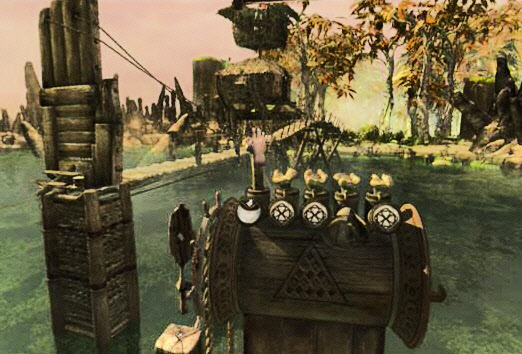
\includegraphics{bonebridge2.jpg}
\caption{Bonebridge puzzle in MYST IV}
\end{figure}

At one time I was a big fan of MYST computer games. I always enjoyed
being lost in a beautiful puzzle which, if you discard the
\emph{beautiful} bit, is a pretty accurate description of my programmer
day job.

\begin{Shaded}
\begin{Highlighting}[]
\NormalTok{bonebridge}\KeywordTok{=:}\NormalTok{3 }\KeywordTok{:} \NormalTok{0}

\CommentTok{NB.*bonebridge  v--  lists  totem  symbol  permutations for  bone}
\CommentTok{NB. bridge.}
\CommentTok{NB.}
\CommentTok{NB. The  solution to  this MYST IV puzzle is similiar to the book}
\CommentTok{NB. shelf puzzle in Tomanha but requires far more  exploration of}
\CommentTok{NB. the age.}
\CommentTok{NB.}
\CommentTok{NB. You are confronted with  5  bones on the lock.  All the bones}
\CommentTok{NB. move independently. You can see the settings for 4 bones. One}
\CommentTok{NB. bone  has a  broken display.  The four  visible bones  have 8}
\CommentTok{NB. symbols on them in the  same order.  The  5th bone also has 8}
\CommentTok{NB. symbols and you can "safely" infer they are in the same order}
\CommentTok{NB. as the visible bones.}
\CommentTok{NB.}
\CommentTok{NB. Four  bone  symbols   match  symbols  found  on  totem  poles}
\CommentTok{NB. distributed around the  age. There is a  5th  totem pole  but}
\CommentTok{NB. fruit eating mangrees  obscure  the  totem symbol and  I have}
\CommentTok{NB. never  seen it.  The  totem  poles are  associated  with  age}
\CommentTok{NB. animals. In addition to the totem poles  there is  a chart in}
\CommentTok{NB. the  mangree  observation  hut  that  displays  a  triangular}
\CommentTok{NB. pattern  of paw  prints.  The  paw  prints  define an  animal}
\CommentTok{NB. ordering. The order  seems to be how  dangerous a  particular}
\CommentTok{NB. animal is;  big scary animals  are at the top and vegetarians}
\CommentTok{NB. are at the bottom.}
\CommentTok{NB.}
\CommentTok{NB. Putting the clues together you infer:}
\CommentTok{NB.}
\CommentTok{NB. a)  the  bridge  combination  is  some  permutation  of  five}
\CommentTok{NB. different symbols}
\CommentTok{NB.}
\CommentTok{NB. b) two possible symbol orders are given by the paw chart}
\CommentTok{NB.}
\CommentTok{NB. c) you know 5 symbols and the 4th is one of the remaining 4}
\CommentTok{NB.}
\CommentTok{NB. If this is  the  case  the number of  possible  lock settings}
\CommentTok{NB. shrinks from 32768 to the ones listed by this verb.}
\CommentTok{NB.}
\CommentTok{NB. monad:  bonebridge uuIgnore}
\CommentTok{NB.}
\CommentTok{NB.   bonebridge 0}

\CommentTok{NB. known in paw order}
\NormalTok{known}\KeywordTok{=.}    \KeywordTok{s:} \StringTok{' square triangle hourglass yingyang'}
\NormalTok{unknown}\KeywordTok{=.}  \KeywordTok{s:} \StringTok{' clover cross xx yy'}

\CommentTok{NB. all possible lock permutations}
\NormalTok{settings}\KeywordTok{=.} \KeywordTok{~.} \NormalTok{5 }\KeywordTok{\{."}\NormalTok{1 tapl known}\KeywordTok{,}\NormalTok{unknown}
\KeywordTok{assert.} \RegionMarkerTok{((}\KeywordTok{!}\NormalTok{8}\RegionMarkerTok{)}\KeywordTok{%!}\NormalTok{8}\KeywordTok{-}\NormalTok{5}\RegionMarkerTok{)} \KeywordTok{=} \KeywordTok{#}\NormalTok{settings}

\CommentTok{NB. possible ordering - we don't know}
\CommentTok{NB. what the fifth symbol is but it}
\CommentTok{NB. occurs in the 3rd slot}
\NormalTok{order}\KeywordTok{=.} \NormalTok{8}\KeywordTok{#s:<}\StringTok{''}
\NormalTok{order}\KeywordTok{=.} \NormalTok{known }\RegionMarkerTok{(}\NormalTok{0 1 6 7}\RegionMarkerTok{)}\KeywordTok{\}} \NormalTok{order}
\NormalTok{order}\KeywordTok{=.} \NormalTok{unknown }\RegionMarkerTok{(}\NormalTok{2 3 4 5}\RegionMarkerTok{)}\KeywordTok{\}} \NormalTok{order}

\CommentTok{NB. keep unknown only in 3rd slot}
\NormalTok{settings}\KeywordTok{=.} \NormalTok{settings }\KeywordTok{#~} \KeywordTok{-.} \KeywordTok{+./"}\NormalTok{1 }\RegionMarkerTok{(}\NormalTok{0 1 3 4}\KeywordTok{\{"}\NormalTok{1 settings}\RegionMarkerTok{)} \KeywordTok{e.} \NormalTok{unknown}
\NormalTok{settings}\KeywordTok{=.} \NormalTok{settings }\KeywordTok{#~} \RegionMarkerTok{(}\NormalTok{2 }\KeywordTok{\{"}\NormalTok{1 settings}\RegionMarkerTok{)} \KeywordTok{e.} \NormalTok{unknown}

\CommentTok{NB. strict row sequence adverb}
\NormalTok{srsm}\KeywordTok{=.}  \NormalTok{1 }\KeywordTok{:} \StringTok{'*./"1 u/&> 2 <\textbackslash{}"1 y'}

\CommentTok{NB. retain strictly increasing and strictly decreasing rows}
\NormalTok{grade}\KeywordTok{=.} \NormalTok{order }\KeywordTok{i.} \NormalTok{settings}
\NormalTok{settings }\KeywordTok{#~} \RegionMarkerTok{((}\KeywordTok{<} \NormalTok{srsm}\RegionMarkerTok{)}\KeywordTok{"}\NormalTok{1 grade}\RegionMarkerTok{)} \KeywordTok{+.} \RegionMarkerTok{(}\KeywordTok{>} \NormalTok{srsm}\RegionMarkerTok{)}\KeywordTok{"}\NormalTok{1 grade}
\RegionMarkerTok{)}
\end{Highlighting}
\end{Shaded}

1 J has its own syntax highlighting tools but they are not part of a
document generation system. pandoc's highlighters elegantly feed into
many output formats making them far more useful.

\end{document}
